\documentclass[12pt]{article}
%% Package imports
\usepackage[utf8]{inputenc}
\usepackage{amsmath}
\usepackage{subcaption}
\usepackage{pgfplotstable}
\usepackage{amsfonts}
\usepackage{amssymb}
\usepackage{graphicx}
\usepackage{physics}
\usepackage[left=2cm,right=2cm,top=2cm,bottom=2cm]{geometry}
\usepackage{multirow}
\usepackage{booktabs}
\usepackage{float}
\usepackage{verbatim}
\usepackage{amsthm}
\usepackage{fancyhdr}
\usepackage[shortlabels]{enumitem}
\renewcommand{\baselinestretch}{1.5}

%% Commands for inserting big braces.
\newcommand\lb{\left\lbrace}
\newcommand\rb{\right\rbrace}

%% Math symbols
\newcommand\Q{\mathbb{Q}}
\newcommand\R{\mathbb{R}}
\newcommand\N{\mathbb{N}}
\newcommand\W{\overline{W}}
\newcommand\intR{\int_{-\infty}^\infty}

\newcommand\st{\text{ such that }}
\parindent 0ex

%% Page style settings
\pagestyle{fancy}
\fancyfoot{}
\fancyhead[L]{\slshape{Probability And Statistics for JMC}}
\fancyhead[R]{\slshape{CID: 01871147}}
\fancyfoot[C]{\thepage}
\begin{document}
\title{Probability And Statistics for JMC Autumn 2021 Coursework}
\date{\today}
\author{Szymon Kubica, CID: 01871147}
\maketitle

\pagebreak
\section*{Question 1.}

\subsection*{(a)}

In order to show that the sample mean of weights, $ \overline{W} $ is an unbiased estimator of the integral $ I $,
we need to show that:
\[ E (\overline{W} | I) = I.\]
Let us consider the left-hand side of the expression above. After using the linearity of expectation, we obtain:
\begin{equation} E (\overline{W} | I) = E\left[ \frac{1}{n}\sum_{i = 1}^n \frac{g(X_i)}{f(X_i)}\right] =\frac{1}{n}\sum_{i = 1}^n  E\left[ \frac{g(X_i)}{f(X_i)}\right]  .\end{equation}

If we now consider the expectation of the weight $ W_i $ above:
\[ E\left[ \frac{g(X_i)}{f(X_i)}\right] = \int_{-\infty}^\infty \frac{g(x)}{f(x)} f(x) dx =\int_{-\infty}^\infty g(x)dx = I. \]
That is because each random variable $ X_i $ is sampled from $ X $ with pdf $ f(x) $ 
and so in order to obtain the expected value of $\dfrac{g(X_i)}{f(X_i)}$ 
we need to integrate over the range $ \mathbb{X} $ while multiplying by the pdf of $ X $
Hence, as shown above the integrand simplifies and we get $ I $.

Now if we substitute what we have established so far back into the equation $(1)$, we get:
\begin{equation} \frac{1}{n}\sum_{i = 1}^n  E\left[ \frac{g(X_i)}{f(X_i)}\right] =\frac{1}{n}\sum_{i = 1}^n  I = \frac{1}{n} n I = I    .\end{equation}

Therefore, we may conclude that $ E (\overline{W} | I) = I $ and hence $ \overline{W} $ is an unbiased estimator of
the integral $ I $. 

\subsection*{(b)}

To show that the variance of this estimator is proportional to $ \left( E\left[\dfrac{g(X)^2}{f(X)^2}\right] - I^2\right)$
let us use the shorthand formula for the variance of a random variable $ X $ which was derived in the lectures:
\[ Var (X) = E (X^2) - (E(X))^2.\]
Applying it to $ \overline{W} $ we obtain:
\[ Var (\overline{W}) = E \left[\left(\frac{1}{n}\sum_{i = 1}^n \frac{g(X_i)}{f(X_i)}\right)^2\right] - (E(\overline{W}))^2. \]
Using previously established fact that the expectation of $ \overline{W} $ is $ I $, and the linearity of 
the expectation we get:
\begin{equation} 
Var (\overline{W}) = \frac{1}{n^2} E \left[\left(\sum_{i = 1}^n \frac{g(X_i)}{f(X_i)}\right)^2\right] - I^2.
\end{equation}

Let us now consider the expectation of the square of the sum of weights, 
multiplying out and applying linearity results in:
\begin{equation}
E \left[\left(\sum_{i=1}^n \frac{g(X_i)}{f(X_i)}\right)^2\right] 
= E \left[\sum_{i = 1}^n \frac{g(X_i)^2}{f(X_i)^2} \right] + \sum_{i=1}^n \sum_{j=1, j \neq i}^n \lb E \left[ \frac{g(X_i)}{f(X_i)} \frac{g(X_j)}{f(X_j)} \right] \rb.
\end{equation}

Now if we focus on the expectation of the product of two weights above, we can treat it as the 
expectation of a product of joint random variables $ \frac{g(X_i)}{f(X_i)} $ and $ \frac{g(X_j)}{f(X_j)}$. We can compute it as follows: 
\[ E \left[ \frac{g(X_i)}{f(X_i)} \frac{g(X_j)}{f(X_j)} \right] 
= \int_{-\infty}^\infty \lb \int_{-\infty}^\infty \frac{g(x)}{f(x)} \frac{g(y)}{f(y)} f(x) dx\rb f(y) dy. \]
Now after simplifying the integrand, and noticing expressions for $ I $ we get: 
\[ \int_{-\infty}^\infty \lb \int_{-\infty}^\infty \frac{g(x)}{f(x)} \frac{g(y)}{f(y)} f(x) dx\rb f(y)dy 
= \int_{-\infty}^\infty \lb \int_{-\infty}^\infty g(x)dx\rb \frac{g(y)}{f(y)} f(y)dy
= I\int_{-\infty}^\infty g(y) dy = I^2. \]

If we now substitute it back into equation $(4)$, we obtain:
\begin{equation} 
E \left[\sum_{i = 1}^n \frac{g(X_i)^2}{f(X_i)^2} \right] + \sum_{i=1}^n \sum_{j=1, j \neq i}^n \lb E \left[ \frac{g(X_i)}{f(X_i)} \frac{g(X_j)}{f(X_j)} \right] \rb 
= E \left[\sum_{i = 1}^n \frac{g(X_i)^2}{f(X_i)^2} \right] + \sum_{i=1}^n \sum_{j=1, j \neq i}^n I^2.
\end{equation}
Now by counting the terms in the double sum, we get:
\[
E \left[\sum_{i = 1}^n \frac{g(X_i)^2}{f(X_i)^2} \right] + \sum_{i=1}^n \sum_{j=1, j \neq i}^n I^2 
= E \left[\sum_{i = 1}^n \frac{g(X_i)^2}{f(X_i)^2} \right] + n (n - 1) I^2. 
\]

After substituting the above result into $ (3) $, we have:
\begin{equation}
  Var (\overline{W}) = \frac{1}{n^2} \left(E \left[\sum_{i = 1}^n \frac{g(X_i)^2}{f(X_i)^2} \right] + n (n - 1) I^2 
 \right) - I^2.
\end{equation}
If we then simplify, it becomes:
\[
  \frac{1}{n^2} \left(E \left[\sum_{i = 1}^n \frac{g(X_i)^2}{f(X_i)^2} \right] + n (n - 1) I^2 \right) - I^2
  =\frac{1}{n^2} \left(E \left[\sum_{i = 1}^n \frac{g(X_i)^2}{f(X_i)^2} \right]\right) + \left( \frac{n(n-1)}{n^2} - 1 \right)I^2.
\]
After further simplification, we obtain:
\begin{equation}
  Var (\overline{W}) 
  =\frac{1}{n^2} \left(E \left[\sum_{i = 1}^n \frac{g(X_i)^2}{f(X_i)^2} \right]\right) - \frac{1}{n}I^2.
\end{equation}

Let us now evaluate the expectation in the bracket above by using linearity and the fact that each $X_i$
is sampled from the same distribution $X$:
\[
  E \left[\sum_{i = 1}^n \frac{g(X_i)^2}{f(X_i)^2}\right]
  = \sum_{i = 1}^n E \left[ \frac{g(X_i)^2}{f(X_i)^2} \right]
  = n E\left[ \frac{g(X)^2}{f(X)^2} \right].
\]
If we now substitute it back into equation $ (7) $, we get the final expression:
\begin{equation}
  Var (\overline{W}) 
=\frac{1}{n} \left(E \left[\frac{g(X)^2}{f(X)^2} \right] - I^2 \right).
\end{equation}

Therefore we deduce that the variance of the estimator $ \overline{W} $ is indeed proportional to 
$ \left(E \left[\dfrac{g(X)^2}{f(X)^2} \right] - I^2 \right) $.
Now if we compute the standard deviation using the formula above, we get:
\begin{equation}
  \sigma (\overline{W}) 
  =\frac{1}{\sqrt{n}} \left(E \left[ \frac{g(X)^2}{f(X)^2} \right] - I^2 \right)^\frac{1}{2}.
\end{equation}
And so the standard deviation is inversely proportional to the square root of the sample size $ n $.

\section*{(c)}

Assume $ g(x) $ was non-negative. In order to show that the choice of the RV $ X $ such that $ f(x) \propto g(x) $ 
makes the variance $ 0 $, let us consider what it means for $ f(x) $ and $ g(x) $ to be proportional.
If they are indeed proportional, then there exists a constant $ k \in \R $ such that:
\[ f(x) = k g(x). \]
Note that the condition $ g(x) $ is non-negative is necessary, because otherwise for positive $ k $, $ f(x) = kg(x) $
wouldn't be a valid pdf as pdf needs to be non-negative.

If we now plug it into our expression for $ \overline{W} $, we get:
\[ \overline{W} = \frac{1}{n} \sum_{i=1}^n \frac{g(X_i)}{f(X_i)} 
= \frac{1}{n} \sum_{i=1}^n \frac{g(X_i)}{kg(X_i)} =\frac{1}{n} \sum_{i=1}^n \frac{1}{k} 
= \frac{1}{n} n \frac{1}{k} = \frac{1}{k}.  \]

Therefore, we deduce that $ \overline{W} $ is a constant RV. Hence, we may compute its variance:
\[ Var(\W) = E\left[(\W - E(\W))^2\right] = E \left[ (\frac{1}{k} - E(\frac{1}{k}))^2 \right]
= E \left[ (\frac{1}{k} - \frac{1}{k})^2 \right] = E (0) = 0.\]

It is impractical to use this "ideal" choice because of the following reasoning. Note that for $ f(x) $ to 
be a valid pdf of the random variable $ X $, it needs to be normalised, i.e. 
\[ \intR f(x)dx = 1,\]
but then also if $ f(x) = kg(x) $, we must have:
\[ \intR kg(x)dx = 1 \iff k = \dfrac{1}{\intR g(x)dx} = I^{-1}. \]
It means that in order to be able to choose $f(x)$ such that it is proportional to $g(x)$, we need to know 
the value of $ I $ to choose the right constant of proportionality. But we don't know it, as we are trying to estimate it.
Hence, even if we were given $f(x)$ which was guaranteed to satisfy the criterion of proportionality, 
our experiment wouldn't make much sense as we could just determine the exact value of $ I $ 
from the constant of proportionality.

\subsection*{(d)}

First let us sample 20 values from  a standard normal distribution using the numpy python library: 
\begin{center}
  \begin{table}[H]\centering
    \pgfplotstableset{
      % global config, for example in the preamble
      % these columns/<colname>/.style={<options>} things define a style
      % which applies to <colname> only.
      every head row/.style={before row=\toprule,after row=\midrule},
      every last row/.style={after row=\bottomrule}
    }
  \pgfplotstabletypeset[% local config, applies only for this table
  1000 sep={\,},
  columns/info/.style={
  fixed,fixed zerofill,precision=2,showpos,
  column type=r,
  }
  ]
  {computations/samples.dat}

  \caption{Sampled Data.}
  \end{table}
\end{center}

In order to compute the estimate of the integral $ I $, I wrote a program in python that took the data and transformed them according to the following procedure. 
Firstly, for each of the sampled values I computed the corresponding weight:
\[ w_i = \frac{g(x_i)}{f(x_i)}\]
Then in order to get the estimate I took the arithmetic mean of the results:
\[ \overline{w} = \frac{1}{n} \sum_{i=1}^n \frac{g(x_i)}{f(x_i)} \]
The obtained value of the estimate for the data above was 1.8380132926975759. 
We can compare it to the actual value of approximately $1.813$. 
Now in order to calculate the $95\%$ confidence interval, we need to assume that the weights are normally distributed. 
Even under this assumption, we still don't know the variance of the distribution of weights, hence we have to estimate it using the bias corrected 
sample variance estimate given by:
\[ S_{n-1}^2 = \frac{1}{n -1} \sum_{i=0}^n(w_i - \overline{w})^2.\]
Now since we are considering a normal distribution with both mean and variance unknown, 
we may use the Student $t$ distribution. 
If we apply a following transformation to $\overline{W}$, we know that:
\[ \frac{\overline{W} - I} {S_{n-1} / \sqrt{n}} \sim \text{Student } t (n - 1)\]
And so in our case, for sample size $ n = 20 $, the $95\%$ confidence interval for $ I $
is given by:
\[ \left[ \overline{w} - t_{19\text{, }0.975} \frac{s_{19}}{\sqrt{20}} \text{, }\overline{w} + t_{19\text{, }0.975} \frac{s_{19}}{\sqrt{20}} \right] \]
Therefore, in order to compute the confidence interval I wrote a function which used python libraries to calculate the respective quantiles of the Student $t$ distribution with 19 
degrees of freedom.
After that, I calculated the bias-corrected sample variance and took a square root of it to get the estimate for the standard deviation $s_{19}$
Then I was able to find the 
$ \delta $ of $t_{19\text{, }0.975} \frac{s_{19}}{\sqrt{20}}$ around the estimate 
$ \overline{w} $. 
Hence by adding and subtracting it, I got the values for the bounds of the interval:
\[ [1.3969120125036336, 2.279114572891518]\]

\subsection*{(e)}
In order to plot the estimated values of $I$ against different values of $\sigma$ for the 
normal distribution of $ X $, I followed the instructions outlined in the coursework specification. I used the matplotlib python library and only needed to modify my code from part $(d)$ slightly in order to allow for changing the standard deviation of the source normal distribution. Each of the red dots in the plot below represents a point estimate of $ I $ for a specific value of $ \sigma $. In addition, each dot has a $95\%$ confidence interval associated with it that was marked in blue. The horizontal line represents the true value of $ I $ equal to 1.81280.

\begin{figure}[H]
  \begin{center}
    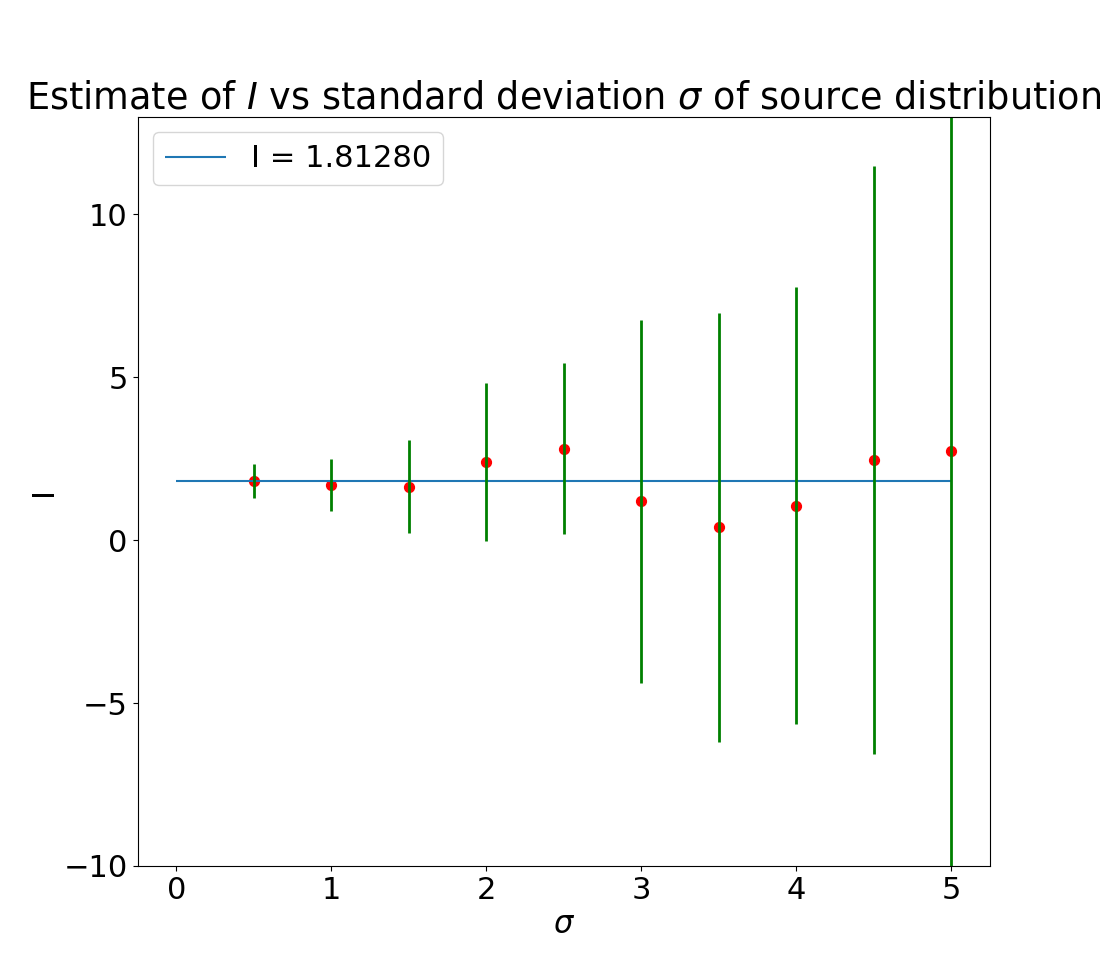
\includegraphics[scale=0.5]{plot1.png}
  \end{center}
\end{figure}

In the figure above, it can be observed that, as the standard deviation of the source distribution increases, the width of the confidence interval also increases. It means that we are less convinced that the real value of $I$ lies close to our estimate, and therefore if we want to find the $95\%$ confidence interval, we need to make it bigger to still be $95\%$
convinced.

\subsection*{(f)}

For part $(f)$ I also wrote a python script that repeated part $(d)$ for $ n = 2^k $ where
$ k = 3, 4, 5, ..., 12 $ 100 times and then computed the standard deviation of those 100 
estimates of $ I $. In order to plot the results as a log-log plot I used matplotlib library. I also added a line given by the equation:
\[ y = \sigma_{n=8} \left( \frac{n}{8} \right)^\lambda,\]
where $\sigma_{n=8}$ is the standard deviation of 100 estimates computed for $ k = 3$. 
And $\lambda$ is the scaling factor of the standard deviation with the sample size $n$ that was predicted in part $(b)$. 
Recall that my result was that the standard deviation scales with a factor of $ \frac{1}{\sqrt{n}} $ and so the value of $ \lambda $ is $ -\frac{1}{2}.$  

\begin{figure}[H]
  \begin{center}
    \hspace*{-1cm}
    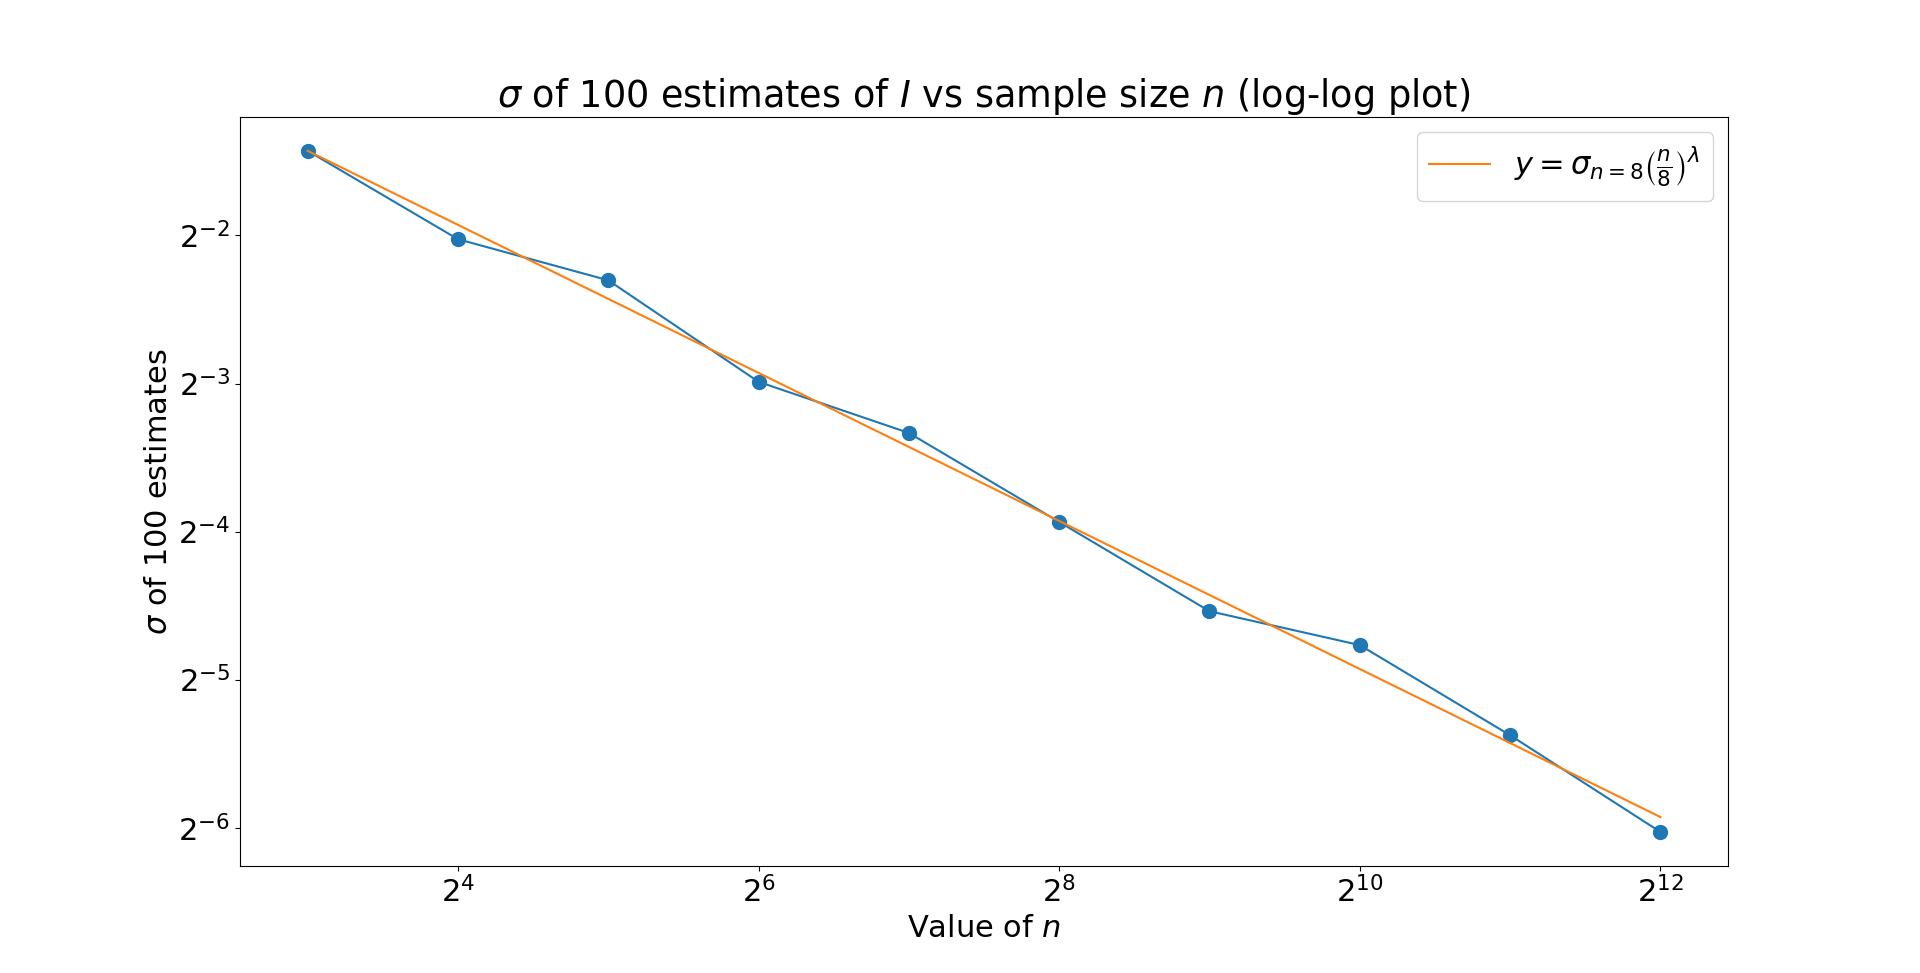
\includegraphics[scale=0.4]{plot2.png}
  \end{center}
\end{figure}
\vspace{-0.75cm}
As we can see the empirical data resulting from repeating the experiment 100 times 
is consistent with the predicted value of $\lambda$. We can clearly observe that as the 
sample size $n$ of the source distribution increases, the standard deviation of our estimator of $ I $ decreases as $ \frac{1}{\sqrt{n}} $ plot.

\subsection*{(g)}

If the pdf $f(x)$ is much narrower or broader than $g(x)$, 
this method becomes unreliable because of the variance of the estimator $\overline{W}$. 
If we consider the expectation in the expression for variance derived in part $(b)$ as an
integral:
\[ E \left[ \frac{g(X)^2}{f(X)^2} \right] = \intR \frac{g(x)^2}{f(x)^2} f(x)dx = \intR \frac{g(x)^2}{f(x)}dx, \]
we may investigate how it changes as we plot the integral for different values of $\sigma$, we can notice that as
$\sigma$ gets very small or very big, we get big peaks on the graph (see figure on the next page). 
If we then try to integrate it, the variance of the estimator will be very big, 
and hence the $95\%$ confidence interval will be very wide,  
which is not useful if we want to estimate the value of $I$ accurately.
\begin{figure}[H]
\centering
\begin{subfigure}{.5\textwidth}
\centering
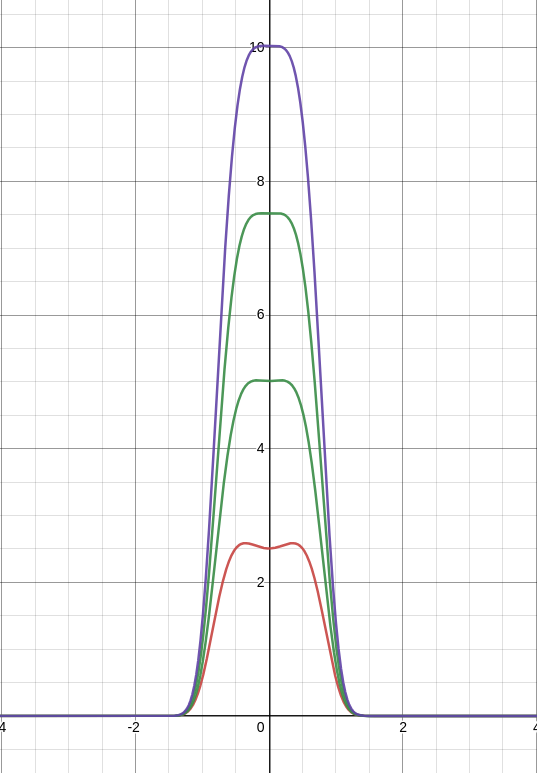
\includegraphics[width=.6\linewidth]{integral1.png}
\caption{$\sigma$ varying from 1 to 4}
\label{fig:sub1}
\end{subfigure}%
\begin{subfigure}{.5\textwidth}
\centering
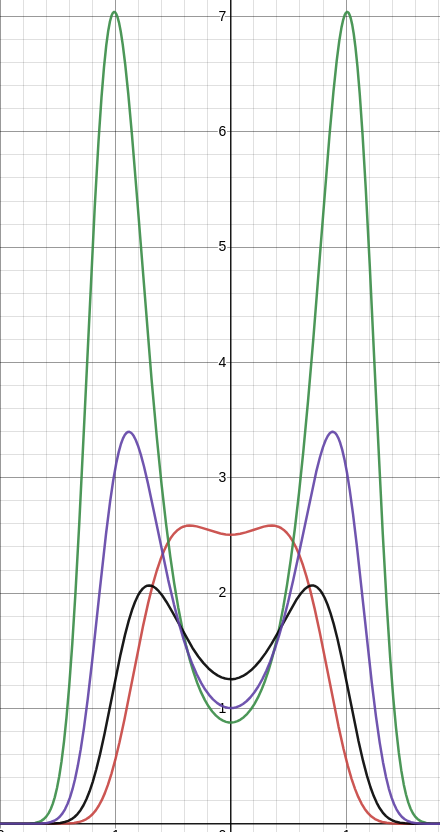
\includegraphics[width=.45\linewidth]{integral2.png}
\caption{$\sigma$ varying from 1 to 0.35}
\label{fig:sub2}
\end{subfigure}
\label{fig:test}
\end{figure}
Note that this reasoning doesn't need to rely on the assumption that $g(x)$ is non-negative. Since we have $ g(x)^2 $ in the integrand, the sign of it doesn't matter. 
The only condition that we need to impose on $g$ is that the integral $I$ needs to be
bounded, so that it makes sense to estimate it. 
Another thing is that we can generalise that reasoning for an arbitrary function $g(x)$,
not necessarily $g(x) = e^{-x^4}$, which was used to plot the graphs above. 
That is because we may motivate our findings by considering what changes to $f(x)$ as we 
tweak the standard deviation. Surely, if we increase it, then the graph of $f$ will be broader but from the normalisation condition it will also become flatter, which means that at the values where $g(x)^2$ is non-zero, the value of $\dfrac{g(x)^2}{f(x)}$ will get bigger and bigger as we divide by values that keep decreasing. 
Similarly, if we decrease the standard deviation of the source distribution, 
it will keep getting narrower and hence the value of f will keep increasing at the mean 
of the distribution, but will keep getting smaller everywhere else, 
that explains why in the second plot above, we have two peaks with a local minimum at 0. 
That is because the distribution even though $f(x)$ increases at the mean point, 
it gets smaller and smaller everywhere else, and so the value of the quotient in the integral will keep getting larger at some points in the range of integration. 

Hence we may deduce that in order for our estimation of $I$ to be as accurate as possible we want to minimise regions of the real line where $f(x)$ is very small whereas $g(x)$ is non-zero, because such intervals cause the value of the variance of our estimator $\overline{W}$ to grow which we want to avoid.
\section*{Question 2.}
Let $ F(x) $ be an arbitrary continuous function that increases monotonically from 0 to 1. If we define the random variable $ X $ by the transformation $ X = F^{-1} (U) $ where 
$ U \sim \text{U}(0, 1) $ we can compute the cdf of $ X $ using its definition as a particular probability:
\[ F_X (x) = P (X \leq x). \]
Now if we substitute our definition of X as a transformation of the uniform distribution, we obtain:
\[P (X \leq x)  = P ( F^{-1} (U) \leq x).\]
Since $ F(x) $ is monotonically increasing from 0 to 1, we may deduce that 
$ F^{-1} (x) $  is well defined and monotonically increasing on interval $ [0,1] $.
Now since U is uniformly distributed between $ 0 $ and $ 1 $, we can conclude:
\[  F^{-1} (U) \leq x \iff U \leq F(x)\]
by applying $ F $ to both sides of the inequality. Hence, coming back to our probability:
\[P ( F^{-1} (U) \leq x) = P (U \leq F(x)),\]
and by definition of the cdf we get:
\[ P (U \leq F(x)) = F_U (F(x)), \]
where $ F_U $ is the cdf of the uniform distribution $ \text{U}(0, 1) $. If we now recall that it is given by:
\[ 
F_U (x) = 
 \begin{cases}
  0, \text{ if } x < 0 \\
  x, \text{ if } 0 \leq x \leq 1 \\
  1, \text{ if } x \geq 1. \\
 \end{cases}
\]

Now since we know that $ F(x) $ increases monotonically between 0 and 1, we know that
$ 0 \leq F(x) \leq 1 $. And so the second case of $F_U$ applies and hence we get:
\[ F_U (F(x)) = F (x). \]

And so after combining all of the above steps together, we may deduce: 
\[  F_X(x) = F(x),  \]
which was to be shown.

\section*{Question 3.}

\subsection*{(a)}

Given that the pmf of the random variable $X$ representing the mass of a random galaxy 
distributed approximately as a power law above the minimum threshold $ x_{min} $ is:
\[ f_X(x) =
  \begin{cases}
    c \left(\frac{x}{x_{min}}\right)^{-\lambda} , \text{ if } x \geq x_{\text{min}} \\
    0,  \text{ if } x \leq x_{\text{min}}
  \end{cases}
\]

We need to show that the constant $ c $ is equal to $ \dfrac{\lambda - 1}{x_{\text{min}}} $, given that $ x_{min} $ is a constant and $ \lambda > 1 $. This can be shown using the normalisation condition for the pmf to be valid, i.e. :
\[ \intR f_X(x) = 1. \] 
If we substitute the definition of $f_X$ into the left hand side of the equation above, we get:
\[ \int_{x_{min}}^\infty  c \left(\frac{x}{x_{min}}\right)^{-\lambda} 
  = \left[ c\left(\frac{x_{\text{min}}}{1 - \lambda}\right) \left(\frac{x}{x_{min}}\right)^{1 - \lambda} \right]_{x_{\text{min}}}^\infty 
  =  c\left(\frac{x_{\text{min}}}{1 - \lambda}\right) (0 - 1^{1 - \lambda})
  = c\left(\frac{x_{\text{min}}}{\lambda - 1}\right)
 \]

 After substituting it back into the initial equation, we get:
 \[c\left(\frac{x_{\text{min}}}{\lambda - 1}\right) = 1 \iff c =\frac{\lambda - 1}{x_{\text{min}}}, \]
 which we needed to show.

 As suggested by the coursework specification, from now on we will set $ x_{\text{min}} = 1$ and so the pdf of our random variable $ X $ is given by:

\[ f_X(x) =
  \begin{cases}
    (\lambda - 1) \left(x\right)^{-\lambda} , \text{ if } x \geq 1 \\
    0,  \text{ if } x \leq 1
  \end{cases}
\]

 \subsection*{(b)}

Now given the measured masses of $ n $ galaxies: $ \underline{x} = (x_1, x_2, ..., x_n)$ we will derive the MLE for $ \lambda $.

Consider the log-likelihood function for the above sample:
\[ l(\lambda | \underline{x}) 
= \sum_{i = 1}^{n} \text{log}\left[ f_{X|\lambda} (x_i) \right]
=\sum_{i = 1}^{n} \text{log}\left[ (\lambda - 1) (x_i)^{-\lambda}  \right]
= n \text{log} (\lambda - 1) - \lambda \sum_{i = 1}^{n} \text{log}(x_i) \]
Now in order to find the $ \lambda $ that maximises the log-likelihood function, we need to look for stationary points of $ l $ by solving the following equation:
\[ \pdv{l}{\lambda} = 0\]
And now if we differentiate $ l $ with respect to $ \lambda $, we get:
\[ \pdv{l}{\lambda} = \frac{n}{\lambda - 1} - \sum_{i = 1}^{n} \text{log} (x_i)\]
And the expression above is 0 iff:
\[ \hat{\lambda} = \left(\frac{1}{n} \sum_{i = 1}^{n} \text{log} (x_i) \right)^{-1} + 1  \]

So we have found the value of $ \lambda $ at which our log-likelihood has a stationary point. Now we need to check the second derivative to see if it is in fact a maximum: 
\[ \pdv[2]{l}{\lambda} = \frac{\partial  }{\partial \lambda} \left(\frac{n}{\lambda - 1} - \sum_{i = 1}^{n} \text{log} (x_i) \right)
= - \frac{n}{(\lambda - 1)^2}\]
And now since $ \lambda > 1 $ we deduce that  
\[- \frac{n}{(\lambda - 1)^2} < 0 \text{ } \forall \text{ } \lambda > 1\] 
And so it must also be negative in particular for our previously derived $ \hat{\lambda} $.
Which means that we have found the maximum likelihood estimate. That is because since log$(x)$ is an increasing function, whichever value maximises the log-likelihood function will also maximise the regular likelihood function.

\subsection*{(c)}
The cdf of the power law distribution is given by:
\[ F_X(x) = \int_{-\infty}^{x} f_X(x)dx 
  \begin {cases}
  0, \text{ if } x \leq 1 \\
  \int_1^x (\lambda - 1) \text{ } x^{-\lambda}dx, \text{ if } x > 1
  \end {cases} 
\]
And the integral from the second case evaluates to:
\[ \int_1^x (\lambda - 1) \text{ } x^{-\lambda}dx 
  = \frac{\lambda - 1}{1 - \lambda} \left[ x^{ 1 - \lambda } \right]_1^x = 1 - x^{1 - \lambda}
\]
Hence, we may deduce that the cdf is given by:
\[ F_X(x) = 
  \begin {cases}
  0, \text{ if } x \leq 1 \\
  1 - x^{ 1 - \lambda} \text{ if } x > 1
  \end {cases} 
\]

Now, clearly the range of $ F_X $ is $ [0, 1] $ and it monotonically increases from 0 to 1 and so if we find its inverse, we can apply the method derived in question 2 to numerically generate samples from $ X $. In order to find the inverse consider:
\[ y = 1 - x^{1 - \lambda} \iff x^{1 - \lambda} = 1 - y \iff x = (1 - y)^{\frac{1}{1 - \lambda}} \]
Hence, we may deduce that:
\[ F^{-1} (x) = (1 -x)^{\frac{1}{1 - \lambda}}\]

\subsection*{(d)}
Having determined the inverse of the cdf of the power law distribution, we can create the density histograms. 
The histograms below were generated according to a following procedure. As outlined in the coursework specification, the script that I wrote to generate the histograms first sampled $ n $ samples of $ X $ using the method from question 2 and a uniform distribution between 0 and 1 from numpy library. 
Then it computed the estimate $ \hat{\lambda}$ by plugging the sample into the estimator:
\[  \left(\frac{1}{n} \sum_{i = 1}^{n} \text{log} (X_i) \right)^{-1} + 1  \]
After that, for each of the 3 cases the script repeated the estimation process $ 10^4 $ times and plotted the histograms using matplotlib. 
The binning of the histograms was chosen as specified in the specification, 
that is for the $ (n, \lambda) = (10, 2) $ and $ (50,4)$ cases I used 90 equally sized bins that cover the interval between 1 and 10, whereas for the $(10, 4)$ case, I used 45 bins of width 0.2 that also covered the interval between 1 and 10. I also added two vertical lines to mark the actual values of $\lambda = 2, \text{4}$ for cases 1 and 2, 3 respectively.

\begin{figure}[H]
  \begin{center}
    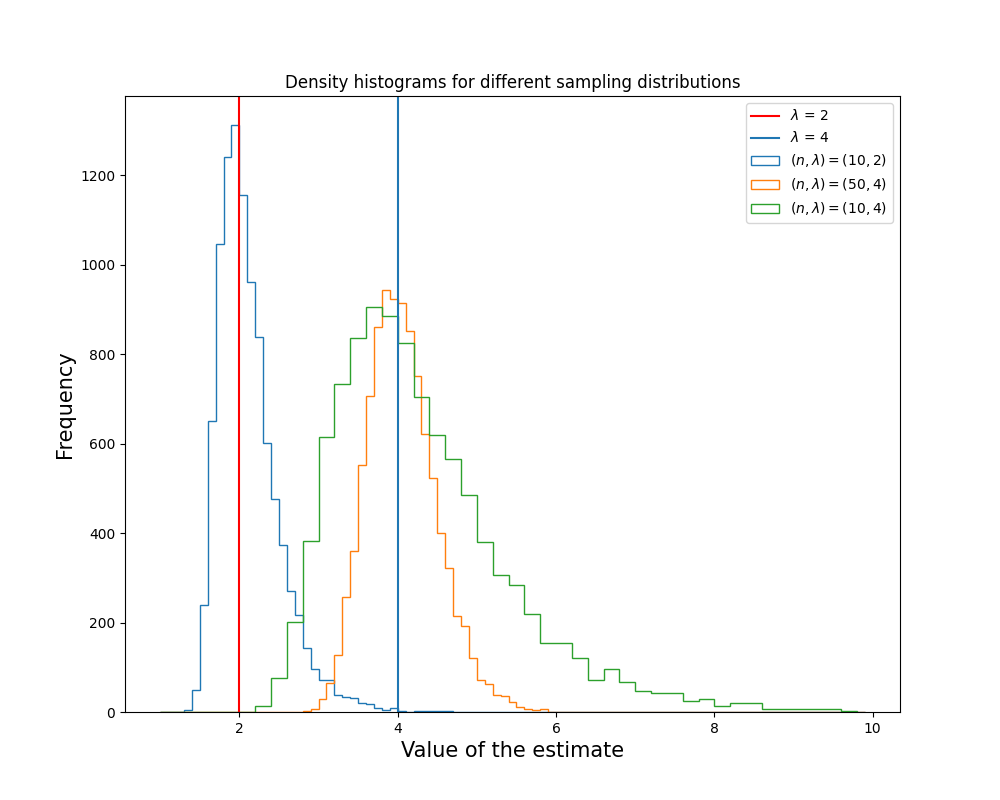
\includegraphics[scale=0.7]{plot3.png}
  \end{center}
\end{figure}

After observing the histograms, case 1 is centered approximately at $ \lambda = 2 $ and hence we may conclude that the estimate value of $ \hat{\lambda} $ is likely to be close to the actual value of $\lambda$. We may state similar observations by focusing on the other two cases, again the largest number of estimates (the peak of the histogram plot) is roughly positioned at the actual value of $\lambda$ parameter. We can also make an additional observation regarding the measure of how those distributions are spread out. Clearly, we can notice that the orange histogram above is much narrower than the green one. An explanation for this is that the orange one which corresponds to the case 2 of the test involved sampling $ n = 50 $ samples as opposed to just 20. Hence the we expect the variance of the estimator to be lower because more samples are taken into account.

\subsection*{(e)}
\subsubsection*{i.}
To determine the appropriate rejection region for our test statistic 
$ T = \hat{\lambda}(X_1, ..., X_n)$ We need to consider what values $ t $ can take and
choose a region of values that are unlikely to occur under $ H_0: \lambda = 2$
Recall that we have derived 
\[ \hat{\lambda} = \left(\frac{1}{n} \sum_{i = 1}^{n} \text{log} (X_i) \right)^{-1} + 1  \]
Where each $ X_i $ must be greater or equal 1 (as $F_X(x) = 0$ if $ x \leq 1$).
Hence, we may deduce that regardless of our sample, the value of our test statistic
$ t $ will always be greater than or equal to 1. N
Let us now consider the form of the alternative hypothesis, i.e $ H_1: \lambda = 4$. We can notice that $H_1$ implies that $ \lambda > 2 $ and so it suffices to carry out a one-sided hypothesis test to test $H_0$ against $H_1$. 
Hence our rejection region will be of a form:
\[[\delta, \infty), \]
where $\delta$ is  some positive constant. Now in order to approximate the rejection region, we might consider the empirical cdf of the data sampled in the histograms. 
By definition, it gives us the proportion of data that is less than or equal to the given input. For large data sets the empirical cdf approximates the actual cdf of the distribution, i.e.:
\[ F_T(t) = P(T \leq t) \approx P(\hat{\lambda_i} < t) = cdf(t), \]
Where $\hat{\lambda_i}$ is any sampled estimate that we computed for part $(d)$ to create the histograms. It means that we can approximate the 
$F_T(t)$ by counting the number of estimates in the histogram that are less than or equal to the given $t$ and then dividing that by the sample size of $10^4$. 
Now, we want to find the rejection region at 5\% level and so if that region is $R$ it must satisfy:
\[ P(T \in R | H_0) = 0.05 \]
Hence in order to find the rejection region so that the Type I error is 5\% I wrote a script which sorted the samples drawn for part $(d)$ for the case of $(n, \lambda) = (10, 2)$ and then picked the sample at index 9500 of the sample array. That way, there are precisely 500 estimates greater 
than that chosen sample and so the probability of $ T $ being greater than that sample is approximately 5\%.

After running the calculation the rejection region that I obtained was:
\[[2.839342235822487, \infty)\]

\subsubsection*{(ii)}
Now the power of the test is defined as the probability that we reject $H_0$ given that $H_1$ is true:
\[ 1 - \beta = P(T \in R | H_1)\]
where $\beta$ is the Type II error rate. 
Now we may approximate it in a similar fashion by counting the number of estimates in the $(n, \lambda) = (10, 4)$ case histogram that fall into the rejection region and dividing the count by the number of sampled estimates.
After running the program to compute the value, the power of the test turned out to be 0.9636 approximately. 

\subsubsection*{(iii)}
Now given the masses observed by the scientists:
\[ \underline{x} = [1.00,\text{ } 1.06,\text{ } 15.69,\text{ } 1.09,\text{ } 4.04,\text{ } 2.20,\text{ } 2.28,\text{ } 1.10,\text{ } 1.46,\text{ } 1.47] \]
we can carry out the hypothesis test by evaluating the estimate using the
formula below and checking if it lands inside of the rejection region. 
\[ \hat{\lambda} = \left(\frac{1}{n} \sum_{i = 1}^{n} \text{log} (x_i) \right)^{-1} + 1  \]

After running the script to compute the estimate, the result was: $2.478118666755411
\approx 2.48. $ Recall that the rejection region defined in 
the previous part was approximately: $[ 2.84, \infty )$. 
Hence, we deduce that the estimated value is outside of the rejection region therefore we retain the hypothesis $ H_0 $.
The $p$ value for an observation is defined as the critical significance 
level at which we have a threshold between rejecting and not rejecting the
null hypothesis. Therefore using our method of approximation, we can 
determine the $p$ value to be the significance level at which our estimate
computed for the data observed by the scientists lies just at the edge of the rejection region. 

Hence, we can compute that critical significance
level by counting the estimates computed in part $(d)$ for the case 1 
, which are greater than or equal to our estimate $ \hat{\lambda} \approx 2.48 $ 

and then dividing the count by the sample size $10^4$ from $(d)$. 
After running the experiment,
the approximate $p$-value turned out to be 0.1469. 
That particular outcome suggests that since the $p$-value is relatively small, even though we didn't reject the null hypothesis, 
there is still relatively strong evidence against it.
That is because, if we were to test at only 15\% significance level, 
we would reject it given the data observed by the scientists.  

\end{document}

